\chapter{Versuchsvorbereitung}


\section{Ziel des Versuchs, Theoretische Grundlagen}
Die Parität galt lange als Erhaltungsgröße, bis 1956 Chien-Shiung Wu mit dem nach ihr benannten Wu-Experiment der Nachweis für die Paritätsverletzung gelang.\\
In diesem Versuch wird die Paritätsverletzung nachgewiesen, indem das nicht-verschwinden eines Pseudoskalars, der Helizität, nachgewiesen wird. Dafür wird über die Polarisation von Bremsquanten die Helizität von Elektronen gemessen, die bei einem $\beta$-Zerfall emittiert werden. 
\subsection{$\beta$-Zerfall}
$\beta$-Zerfälle sind Kernzerfälle, bei denen die Massenzahl des Kerns erhalten bleibt, die Ordnungszahl aber um eins erhöht oder erniedrigt wird. Der $\beta$-Zerfall ist für dieses Experiment relevant, da er Prozess der schwachen Wechselwirkung ist und sich somit zur Untersuchung der Paritätsverletzung eignet. Die verschiedenen Fälle dieser Zerfallsart werden im folgenden erläutert.
\subsubsection{$\beta^+$-Zerfall}
Beim $\beta^+$-Zerfall zerfällt ein Proton in ein Neutron, ein Positron und ein Elektron-Neutrino.
$${}_{{1}}^{{1}}{\mathrm {p}}\to {}_{{0}}^{{1}}{\mathrm {n}}+{\mathrm {e}}^{{+}}+\nu _{e}$$

\subsubsection{$\beta^-$-Zerfall}
Beim $\beta^-$-Zerfall zerfällt ein Neutron in ein Proton, ein Elektron und ein Elektron-Antineutrino.
$${}_{{0}}^{{1}}{\mathrm {n}}\to {}_{{1}}^{{1}}{\mathrm {p}}+{\mathrm {e}}^{{-}}+\overline {\nu }_{e}$$
\subsubsection{Elektroneneinfang}
Der Elektroneneinfang wird zu den $\beta$-Zerfällen gezählt, obwohl dabei keine $\beta$-Strahlung emittiert wird. Hier wird ein Proton des Kerns in ein Neutron umgewandelt. Dabei wird ein Elektron einer kernnahen Schale zerstört und ein Neutrino erzeugt und emittiert. 
$${\displaystyle {}_{Z}^{A}\mathrm {X} +\mathrm {e} ^{-}\to {}_{Z-1}^{A}\mathrm {Y} \mathrm {+} \nu _{e}}$$

\subsubsection{Zerfall eines freien Neutrons}
Ein freies Neutron kann zerfallen. 
$${\hbox{n}}\to {\hbox{p}}+{\hbox{e}}^{-}+\overline {\nu }_{{{\mathrm {e}}}}$$
Die Lebensdauer eines freies Neutrons ist allerdings deutlich größer als die durchschnittliche Zeitdauer bis zur Aufnahme des Neutrons in einen Atomkern, wodurch dieser Zerfall selten eine Rolle spielt.
\subsubsection{Inverser $\beta$-Zerfall}
Beim inversen $\beta$-Zerfall wird ein Proton durch Reaktion mit einem Neutrino in ein Neutron und Positron umgewandelt.
$${\displaystyle \mathrm {p} +{\overline {\nu }}_{e}\to \mathrm {n} +\mathrm {e} ^{+}}$$
Durch diesen Zerfall gelang 1956 der erste experimentelle Neutrinonachweis.

\subsection{Parität und Pseudoskalare}

Der Paritätsoperator erwirkt eine Inversion der Koordinaten. 
$$P\Psi_{(\vec{r})} = \Psi_{(-\vec{r})}$$
Die Paritätsoperation ist einer Spiegelung und nachfolgender Drehung um $180^\degree$ äquivalent.
Da die zweifache Anwendung des Paritätsoperators auf einen Zustand wieder den Zustand selbst ergibt, sind die Eigenwerte einfach zu ermitteln:
$$P^2 = 1 \quad P = P^{-1} $$
$$P^2\ket{a} = \ket{a} = \pi_a^2\ket{a}$$
$$\rightarrow \pi_a = \pm 1$$

Der Erwartungswert eines beliebigen Operators mit definierter Parität transformiert sich unter der Paritätsoperation also wie
$$POP^{-1} = \pi_0 0$$
das heißt das Vorzeichen bleibt entweder erhalten oder ändert sich. 
Operatoren deren Erwartungswert das Vorzeichen ändert, sind unter dieser Transformation nicht invariant. Sie werden durch polare Vektoren beschrieben. Beispiele hierfür sind der Orts- und Impulsoperator.\\
Operatoren deren Erwartungswert das Vorzeichen nicht ändert, sind unter dieser Transformation invariant. Sie werden axiale Vektoren beschrieben. Beispiele hierfür sind der Drehimpuls- und Spinoperator. 
Die Paritätserhaltung beschreibt die Invarianz des Erwartungswerts eines Operators gegen Raumspiegelungen. Um die Paritätserhaltung zu prüfen, werden Operatoren gemessen, die empfindlich auf diese Raumspiegelung sind. Diese Operatoren nennt man Pseudoskalare. Sie entstehen aus dem Skalarprodukt eines axialen und eines polaren Vektors. Ist die Parität erhalten, sind diese Pseudoskalare immer notwendigerweise gleich Null. 
$$\braket{a} = \braket{PaP} = \braket{-a} \rightarrow a = 0$$
Ein von Null verschiedener Pseudoskalar bedeutet somit die Verletzung der Parität.
In diesem Versuch wird der Helizitätsoperator $H$ als Pseudoskalar untersucht. 
$$ H = \frac{\vec{\sigma}\cdot\vec{p}}{\left\vert\vec{\sigma}\cdot\vec{p}\right\vert}$$


\subsection{Polarisation}
Die Polarisierung eines Teilchens in Richtung einer ausgezeichneten Achse ergibt sich aus dem Verhältnis des Erwartungswert des Spins in diese Richtung zum Betrag des Gesamtspins. Im Falle eines Elektrons lassen sich nur die die beiden Zustände $\ket{+}$ und $\ket{-}$ (parallel und antiparallel zur ausgezeichneten Achse) mit den Wahrscheinlichkeiten $a_+$ und $a_-$ messen. 
$$\ket{\Psi} = a_+\ket{+} + a_-\ket{-}$$
Daraus folgt für die Polarisation
$$P = \frac{\bra{\Psi} S_z  \ket{\Psi}}{S} = a_+^2 - a_-^2$$

Die Polarisation von mehreren Teilchen ergibt sich aus der Mittelung über die Einzelpolarisationen. 
$$P = \Bar{\frac{{\braket{S_z}}}{S}} = \sum_{S_z = -1/2}^{S_z=1/2} p_{S_z} \bra{S,S_z}\sigma_z\ket{S,S_z}$$
mit den normierten Wahrscheinlichkeiten $p_{1/2} = p_+$ und $p_{-1/2}= p_-$ für das Auftreten eines reinen Zustandes mit einem bestimmten $S_z$. Benutzt man die Basiszustände (1,0) und (0,1) und die Paulimatrizen als Darstellung der Spinoperatoren, so ergibt sich 
$$P = p_+ - p_-$$
Die Wahrscheinlichkeiten $p_+$ und $p_-$ lassen sich durch zählen der Teilchen im jeweiligen Zustand ermitteln. Somit ergibt sich die Polarisation zu
$$P = \frac{N_+ - N_-}{N_+ + N_-}$$
wobei $N_\pm$ die Anzahl der Elektronen im Zustand $\ket{\pm}$ repräsentiert. Diese Gleichung ist allerdings nur im nicht-relativistischen Grenzfall gültig, da Spin und Drehmoment i.A. gekoppelt sind. 

Anders als das Elektron hat ein Gammaquant den Spin 1. Im Allgemeinen resultieren daraus drei mögliche Ausrichtungen des Spins, da sich das Photon allerdings mit Lichtgeschwindigkeit bewegt, gibt es keinen transversalen Spin. Somit kann der Spin nur parallel oder antiparallel zur ausgerichtet sein. Dies entspricht der rechts- bzw. linkszirkular Polarisation der klassischen Optik. Ein einzelnes Gammaquant ist immer zirkular polarisiert, somit genügt es zur Beschreibung der Polarisation der Gesamtheit der Gammaquanten, die Wahrscheinlichkeiten anzugeben, mit denen die reinen Zustände vorliegen. Dies führt zu einer analogen Formel.
$$P_G = \frac{N_+ - N_-}{N_+ + N_-}$$
wobei $N_\pm$ die Anzahl der rechts-/linkszirkular polarisierten Gammaquanten repräsentiert. 

\section{Experimenteller Aufbau und Messprinzip}
\subsection{Aufbau}
\begin{figure}[H]
    \centering
    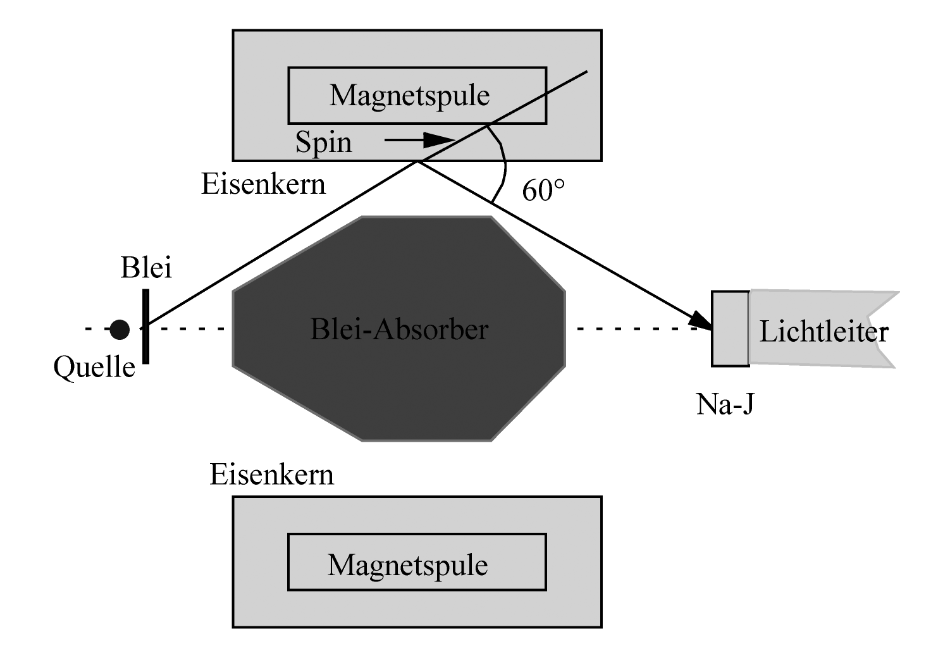
\includegraphics[width=110mm,scale=0.5]{Paritaetsverletzung/include/ParitaetsverletzungAufbau.png}
    \caption{Skizze des Versuchaufbaus aus der Blauen Buch \cite{BlueBook}} 
    \label{fig:Versuchsaufbau}
\end{figure}
Der Versuch ist \ref{fig:Versuchsaufbau} entsprechend aufgebaut. Die Quelle ist eine radioaktive $^{90}Sr^{90}Y$-Quelle, in der Strontium in Yttrium zerfällt, und Yttrium über einen $\beta^-$-Zerfall in Zirconium. Vor der Quelle befindet sich eine dünne Bleischicht, welche die vom Zerfall emittierten Elektronen abbremst und somit Bremsquanten erzeugt. Dahinter befindet sich eine Anordnung aus einem Bleiabsorber und Eisenkernen, deren Geometrie es nur Bremsquanten, die im 60\degree Winkel vom Eisenkern gestreut haben, ermöglicht den dahinter liegenden Na-J-Detektor zu erreichen. Die Eisenkerne selbst enthalten eine Magnetspule, über die der Eisenkern magnetisiert werden kann. Das Signal des Detektors wird über eine langen Lichtwellenleiter an einen Photomultiplier weiter geleitet, der sicher außerhalb des Störungsreichweite des Magnetfelder der Eisenkerne liegt. Der Photomultiplier selbst verstärkt das eingehende Signal, sodass es von einem angeschlossenem Zähler registiert werden kann. 
\subsection{Übertrag der Helizität}
Bei der Erzeugung der Bremsquanten wird ein Teil der Polarisation der Elektronen aus die Bremsquanten übertragen. Somit ist es möglich, aus der Messung der Polarisation der Bremsquanten auf die Polarisation der Elektronen zu schließen. 

Bei diesem Übertrag der Polarisation ergeben sich drei Fälle, abhängig von der Ausgangspolarisation der Elektronen. 
\begin{itemize}
    \item \textbf{unpolarisierte Elektronen} führen zu linear polarisierter Bremsstrahlung. Die Polarisation ist bei geringer Photonenenergie am höchsten und verschwindet bei hoher Photonenenergie.
    \item \textbf{transversal polarisierte Elektronen} führen zu elliptisch polarisierter Bremsstrahlung. Der Betrag der Polarisierung verhält sich wie im Fall darüber.
    \item \textbf{longitudinal polarisierte Elektronen} führt zu zirkular polarisierter Bremsstrahlung. Die Polarisation ist immer größer als im zweiten Fall und stiegt mit der Energie. Hat das Elektron eine negative Helizität, wird ein linkszirkular polarisierter Bremsquant erzeugt.
\end{itemize}
    In diesem Experiment ist nur der letzte Fall relevant. Da Helizität des Elektrons und die zirkulare Polarisation der Bremsquanten immer das gleiche Vorzeichen haben, kann davon ausgegangen werden das durch den Bremsvorgang Helizität übertragen wird. Dieser Helizitätsübertrag kann mit der Abbildung 7.7 des blauen Buches \cite{BlueBook} abgeschätzt werden. In diesem Versuch werden Photonen erst ab einer Energie von \SI{1}{MeV} gemessen. 
    Die Helizität der Elektronen ergibt sich dann zu
    \begin{equation}
        H = \frac{P_G}{L}
        \label{Helizität}
    \end{equation}
    wobei L der Helizitätsübertrag ist. 


\subsection{Messung der Polarisation von $\gamma$-Quanten durch Comptonstreuung}
Die longitudinale Polarisation der Photonen kann durch Comptonstreuung an spinpolarisierten Elektronen gemessen werden, da der Compton-wirkungsquerschnitt mitunter von der Polarisation $P_G$ abhängt. 
$$\odv{\sigma}{\Omega} = \frac{r_0^2}{2} \cdot \frac{k^2}{k_0} \cdot (\Phi_0 + f \cdot P_G \cdot \Phi_C)  $$
Dabei ist $r_0$ der Elektronenradius, $k_0$ der Impuls des Einfallenden Photons, $k$ der Impuls des gestreuten Photons und $f$ der Polarisationsgrad der Elektronen. In diesem Experiment gilt $f = \frac{2}{26}$, da magnetisiertes Eisen als Streutarget verwendet wird. 
$\Phi_0$ ist dabei der Spin unabhängige Teil und beeinhaltet die Abhängigkeit des Wirkungsquerschnitts vom Streuwinkel $\Theta$
$$\Phi_0 = 1 + \cos{\Theta}^2 + (k_0 - k)\cdot (1-\cos{\Theta})$$
$\Phi_C$ ist der polarisationsabhängige Teil
$$\Phi_C = -(1 -\cos{\Theta}) \cdot (k_0 + k) \cos{\Theta} \cos{\Psi}+ k \sin{\Theta} \sin{\Psi} \cos{\Phi}$$ 
Dabei ist $\Psi$ der Winkel zwischen dem Impuls des Einfallenden Photons und dem Elektronenspin, $\Phi$ der Winkel zwischen der $(\Vec{k_0}\cdot\Vec{S})$ Ebene und der $(\Vec{k_0}\cdot\Vec{k})$ Ebene.
Ändert sich der Elektronenspin, ändert sich auch das Vorzeichen von $\Phi_C$, das der Winkel $\Psi$ sich zu $\Psi + \pi$ ändert. Deswegen definiert man sich $\Psi_0$ für die beiden Bereiche $0 \leq \Psi \leq \frac{\pi}{2}$ und $\pi \leq \Psi \leq \frac{3\pi}{2}$ zu $\Phi_C^\pm$. In Bezug auf diese Bereiche werden auch $N_+$ und $N_-$ definiert, als Anzahl an der Photonen mit Polarisation in, bzw. gegen Spinrichtung. Das Verhältnis des Zählrate ergibt sich zu 
$$\frac{N_+ - N_-}{N_+ + N_-} = f \cdot P_G \cdot \frac{\Phi_C^-}{\Phi_0} = E$$
Die Asymmetrie $E$ kann vergrößert werden, indem man den Faktor $\frac{\Phi_C^-}{\Phi_0}$ durch optimale Einstellungen maximiert. Somit werden in diesem Experiment nur Photonen mit einer Energie von $> \SI{1}{MeV}$ unter einem Einfallswinkel von $60 \degree$ gezählt. Damit ergibt sich laut dem blauen Buch zu $\frac{\Phi_C^-}{\Phi_0} = 0.52 \pm 0.05$. \cite{BlueBook} 
Mit der Asymmetrie kann die zirkulare Polarisation $P_G$ der Gammaquanten bestimmt werden. 
\begin{equation}
    P_G = \frac{E}{f}\cdot \frac{\Phi_0}{\Phi_C^-}
    \label{Polarisation}
\end{equation}
\section{Durchführung}
\subsection{Kalibrierung}
Um den im Detektor enthaltenen Diskriminator so einzustellen, das nur Bremsquanten gezählt werden, eine Anfangsenergie von $\SI{1}{MeV}$ haben, muss dieser kalibriert werden. Die Bremsquanten geben durch die Comptonstreuung einer Teil ihrer Energie ab. 
$$E' = \frac{E_0}{\frac{E_0}{m_ec^2}\cdot(1-\cos{\Theta})+1}$$
Bei einer Anfangsenergie von $\SI{1}{MeV}$ und einem Einfallswinkel von $60\degree$ ergibt sich einer Restenergie von etwa $\SI{505}{keV}$. Um den Diskriminator auf etwa diese Energie zu kalibrieren, verwenden wir ein $^{22}$Na-Präparat. Natrium ist zerfällt durch einen $\beta^+$-Zerfall in $^{22}$Ne und lässt dabei ein Positron frei. Dieses Positron annihiliert mit einem Elektron in der Umgebung und erzeugen zwei Photonen mit einer Energie von $\SI{511}{keV}$, unter der Voraussetzung das die beiden Teilchen zuvor eine vernachlässigbare kinetische Energie hatten. Der Diskriminator wird nun so eingestellt, das dieser $\SI{511}{keV}$-Peak gerade noch sichtbar ist. Somit ist sichergestellt das nur Photonen mit einer Anfangsenergie von $>\SI{1}{MeV}$ gezählt werden.
\subsection{Hintergrundmessung}
Eine Messung der Hintergrundaktivität ist aufgrund der geringen Energie der Hintergrundphotonen nicht nötig und wird in diesem Versuch nicht durchgeführt.
\subsection{Messung}
Es werden die Anzahl an Photonen gemessen, die genug Energie haben um den Diskriminator zu überwinden. Dies wird für jede der beiden Spinpolarisierungseinstellungen der Elektronen im Eisenkern 30 Mal für 30 Sekunden durchgeführt. Die Spinpolarisierung der Elektronen im Eisenkern wird geändert, indem die Magnetpule umgepolt wird. Damit sind nun Messwerte für $N_-$ und $N_+$ verfügbar. Daraus lassen sich mit den Formeln \ref{Helizität} und \ref{Polarisation} die Helizität berechnen. Ist diese nicht gleich Null, ist die Paritätserhaltung verletzt. 